% Options for packages loaded elsewhere
\PassOptionsToPackage{unicode}{hyperref}
\PassOptionsToPackage{hyphens}{url}
%
\documentclass[
]{article}
\usepackage{amsmath,amssymb}
\usepackage{lmodern}
\usepackage{iftex}
\ifPDFTeX
  \usepackage[T1]{fontenc}
  \usepackage[utf8]{inputenc}
  \usepackage{textcomp} % provide euro and other symbols
\else % if luatex or xetex
  \usepackage{unicode-math}
  \defaultfontfeatures{Scale=MatchLowercase}
  \defaultfontfeatures[\rmfamily]{Ligatures=TeX,Scale=1}
\fi
% Use upquote if available, for straight quotes in verbatim environments
\IfFileExists{upquote.sty}{\usepackage{upquote}}{}
\IfFileExists{microtype.sty}{% use microtype if available
  \usepackage[]{microtype}
  \UseMicrotypeSet[protrusion]{basicmath} % disable protrusion for tt fonts
}{}
\makeatletter
\@ifundefined{KOMAClassName}{% if non-KOMA class
  \IfFileExists{parskip.sty}{%
    \usepackage{parskip}
  }{% else
    \setlength{\parindent}{0pt}
    \setlength{\parskip}{6pt plus 2pt minus 1pt}}
}{% if KOMA class
  \KOMAoptions{parskip=half}}
\makeatother
\usepackage{xcolor}
\usepackage[margin=1in]{geometry}
\usepackage{graphicx}
\makeatletter
\def\maxwidth{\ifdim\Gin@nat@width>\linewidth\linewidth\else\Gin@nat@width\fi}
\def\maxheight{\ifdim\Gin@nat@height>\textheight\textheight\else\Gin@nat@height\fi}
\makeatother
% Scale images if necessary, so that they will not overflow the page
% margins by default, and it is still possible to overwrite the defaults
% using explicit options in \includegraphics[width, height, ...]{}
\setkeys{Gin}{width=\maxwidth,height=\maxheight,keepaspectratio}
% Set default figure placement to htbp
\makeatletter
\def\fps@figure{htbp}
\makeatother
\setlength{\emergencystretch}{3em} % prevent overfull lines
\providecommand{\tightlist}{%
  \setlength{\itemsep}{0pt}\setlength{\parskip}{0pt}}
\setcounter{secnumdepth}{-\maxdimen} % remove section numbering
\ifLuaTeX
  \usepackage{selnolig}  % disable illegal ligatures
\fi
\IfFileExists{bookmark.sty}{\usepackage{bookmark}}{\usepackage{hyperref}}
\IfFileExists{xurl.sty}{\usepackage{xurl}}{} % add URL line breaks if available
\urlstyle{same} % disable monospaced font for URLs
\hypersetup{
  pdftitle={Report of the results : carbon accounting and choice of indicators},
  pdfauthor={Léa Settepani},
  hidelinks,
  pdfcreator={LaTeX via pandoc}}

\title{Report of the results : carbon accounting and choice of
indicators}
\author{Léa Settepani}
\date{2022-07-29}

\begin{document}
\maketitle

The primary goal of carbon accounting is to establish a measure of how
much greenhouse gases (GHG) are emitted by which actors. The level can
be regional (comparing groups of countries), national (comparing
countries), sectoral (comparing products or aggregate sectors) or
individual (comparing firms for example). Beyond the methodological
concerns, it is important to state what the use of these indicators is.
It is both a descriptive and a normative question. On the one hand, the
need for action against climate change commands to have a clear view of
the global situation. Hence the need for accurate measurements of carbon
emissions as a descriptive concern. On the other hand, this situation
also requires to identify policy strategies to avoid dramatic
consequences on ecosystems. Hence the normative concern and the need to
identify whom should take actions. This second question relates to the
question of responsibility and is much less easy to solve:
responsibility is preceded by ethics and morals, and triggers corrective
actions as consequences. This makes social and political acceptability
crucial. The contribution of research in this debate is at the core of
the question in order to legitimate carbon accounting measures.

This report rather situates itself on descriptive grounds. It includes a
summary of the state of the art in terms of approaches and methods, as
well as the computations of three indicators.

intro meta sur la question de la resp, contextualiser rappel des
concepts et la problématique

\hypertarget{litterature-review-carbon-accounting-methods}{%
\section{Litterature review (carbon accounting
methods)}\label{litterature-review-carbon-accounting-methods}}

This litterature review aims at presenting the various methods that can
be used for carbon accounting, with the underlying question of how to
use them to solve market failures (externalities).

\hypertarget{description-of-the-empirical-strategy}{%
\section{Description of the empirical
strategy}\label{description-of-the-empirical-strategy}}

\hypertarget{the-data}{%
\subsection{The data}\label{the-data}}

Exiobase data was used within an input-output model.

Economic and demographic data from Eurostat was added to custom the
indicators and graphs and allow to draw conclusions more easily.

\hypertarget{method-and-indicators}{%
\subsection{Method and indicators}\label{method-and-indicators}}

\hypertarget{formulas-from-the-input-output-model-to-carbon-accounting}{%
\subsubsection{Formulas: from the input-output model to carbon
accounting}\label{formulas-from-the-input-output-model-to-carbon-accounting}}

The Leontief matrix (\(A\)) is computed by the usual formula
\(A=Z\hat{X}^{-1}\) (\(Z\) is the square matrix of intermediate
consumptions and \(X\) is the total production vector). So \(A\) is the
square\footnote{\(X\) is diagonalized so that \(\hat{X}\) is a square
  matrix} matrix of technical coefficients since it gives the amount of
direct inputs needed to produce one unit of output. The Leontief inverse
\(L\) is obtained by \(L=(I-A)^{-1}\). It is the matrix of total
requirements: the amount of direct and indirect inputs needed to produce
one unit of output.

We can find back the accounting equality \(X=LY\) where \(Y\) is final
demand\footnote{The value of production is the sum of the value of
  inputs and of final demand}. We can also find the vector of
value-added by subtracting inputs from production (\(V=X-Z\bf{1}\) where
\(\bf{1}\) is a vector of 1).

This is the basis of the computations to find the indicators of
environmental impact. The emissions coefficients\footnote{quote
  litterature that talks about ``emissions coefficients''} for the
producer (\(S\)) are obtained by dividing total emissions by the value
of production: \(S=FX^{-1}\). For the value-added approach, which is
also a producer approach, the production vector is replaced by the
value-added vector (\(S_{VA}=FV^{-1}\)). The emissions coefficients for
the consumer (\(M\)) are obtained by multiplying the producer's
coefficients by the Leontief inverse: \(M=SL\). According to this
formula, the consumer (or demand) coefficients take into account the
imported emissions of each sector.

To obtain the total emissions attributed to the producer or to demand,
the emissions coefficients are multiplied by the corresponding economic
volume: \(S_{volume}=S\hat{X}\), \(S_{VA,volume}=S\hat{V}\) and
\(M_{volume}=M\bf{\hat{y}\) (\(\bf{\hat{y}\) is)

\hypertarget{the-resulting-indicators}{%
\subsubsection{The resulting
indicators}\label{the-resulting-indicators}}

Indicators of environmental impact in PBE and VBE are equal in volume
because VBA is closely related to PBA.

Even if the total emissions by sector or country have the same,
environmental multiplicators (volume of emissions normalized by the
value of production or value-added) are different. Not only do they
reflect that wealth creation is more emissions-intensive (mechanically
since VA\textless production) but also that some sectors or countries
benefit much more from emissions than what can be seen by just looking
at volumes.

\hypertarget{visualisation-and-analysis-of-the-ruxe9sults}{%
\section{Visualisation and analysis of the
résults}\label{visualisation-and-analysis-of-the-ruxe9sults}}

\hypertarget{the-global-scale-setting-the-big-picture}{%
\subsection{The global scale (setting the big
picture)}\label{the-global-scale-setting-the-big-picture}}

QUELLE REPARTITION ENTRE REGIONS CHOISIR ??

\begin{figure}
\centering
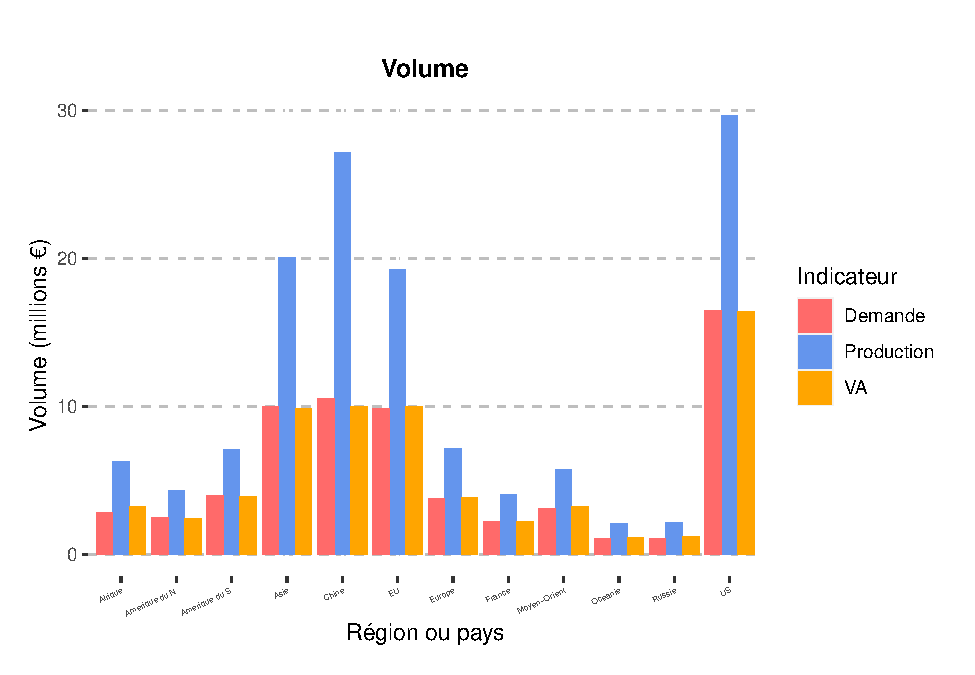
\includegraphics{resultatsEU2_files/figure-latex/monde pays-1.pdf}
\caption{A CHANGER SELON CHOIX REGIONS}
\end{figure}

(DIFFERENCE ENTRE DEMANDE ET VA = STOCKS ?)

Countries that produce (and demand) the most are the US and China,
followed by other Asian countries and EU. When looking at aggregate
world regions, Asia (including China) has by far the largest
environmental impact: three times as large as the second largest impact
(North America). The smallest impact is attributed to Oceania (and the
second smallest to South America).

Regions can be divided into two groups: net exporters of GHG emissions
(Africa, Asia, Middle East) and net importers of GHG emissions (America
and Europe) \footnote{Oceania's situation is roughly balanced.}.

Inequalities in environmental impact are larger with PBE (or VBA) than
with CBA. But regardless of the approach chosen, the attribution of
responsibility preserves the same ranking across regions.

\begin{figure}
\centering
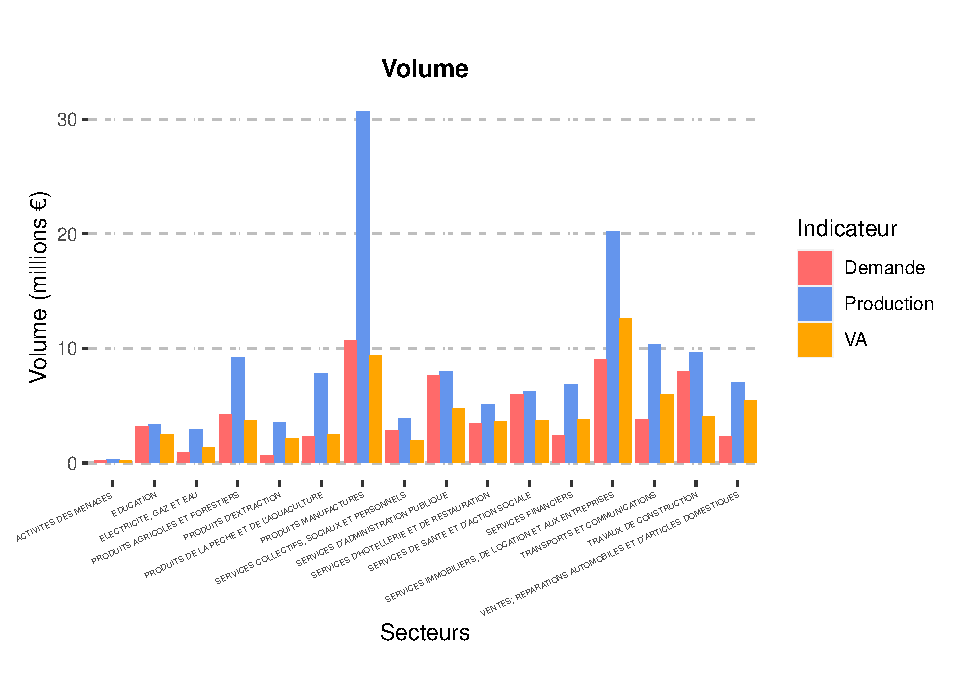
\includegraphics{resultatsEU2_files/figure-latex/monde secteurs volume-1.pdf}
\caption{Des inégalités d'impacts qui varient selon l'approche choisie}
\end{figure}

The repartition between sectors is very different because the sectors
that produce (and demand) the most are not those with the largest
impact.

The sector producing and demanding the most is ``PRODUITS
MANUFACTURES'', but ``ELECTRICITE, GAZ ET EAU'' has the largest
environmental impact (coming from the fact that in this sector each unit
of production is much more emissions-intensive). However, ``PRODUITS
MANUFACTURES'' still has the largest environmental impact in CBA, and
the second largest in CBA. ``TRAVAUX DE CONSTRUCTION'' and
``ELECTRICITE, GAZ ET EAU'' come next in CBA, with impacts half as large
(4 Gt CO2eq) as ``PRODUITS MANUFACTURES'' (8 Gt CO2eq). Transports and
the primary sector (``PRODUITS AGRICOLES ET FORESTIERS'', PRODUITS
D'EXTRACTION'' and ``PRODUITS DE LA PECHE ET DE L'AQUACULTURE'') also
have relativley high environmental impacts (2 to 3 Gt CO2eq) in PBA
while services have low impacts. In CBA, the primary and tertiary
sectors range from 0 to 2 Gt CO2eq, with not particular pattern.

One feature that is similar to the regional approach above is that
impacts are more uneven in the PBA and VBA approaches than in CBA.

\begin{figure}
\centering
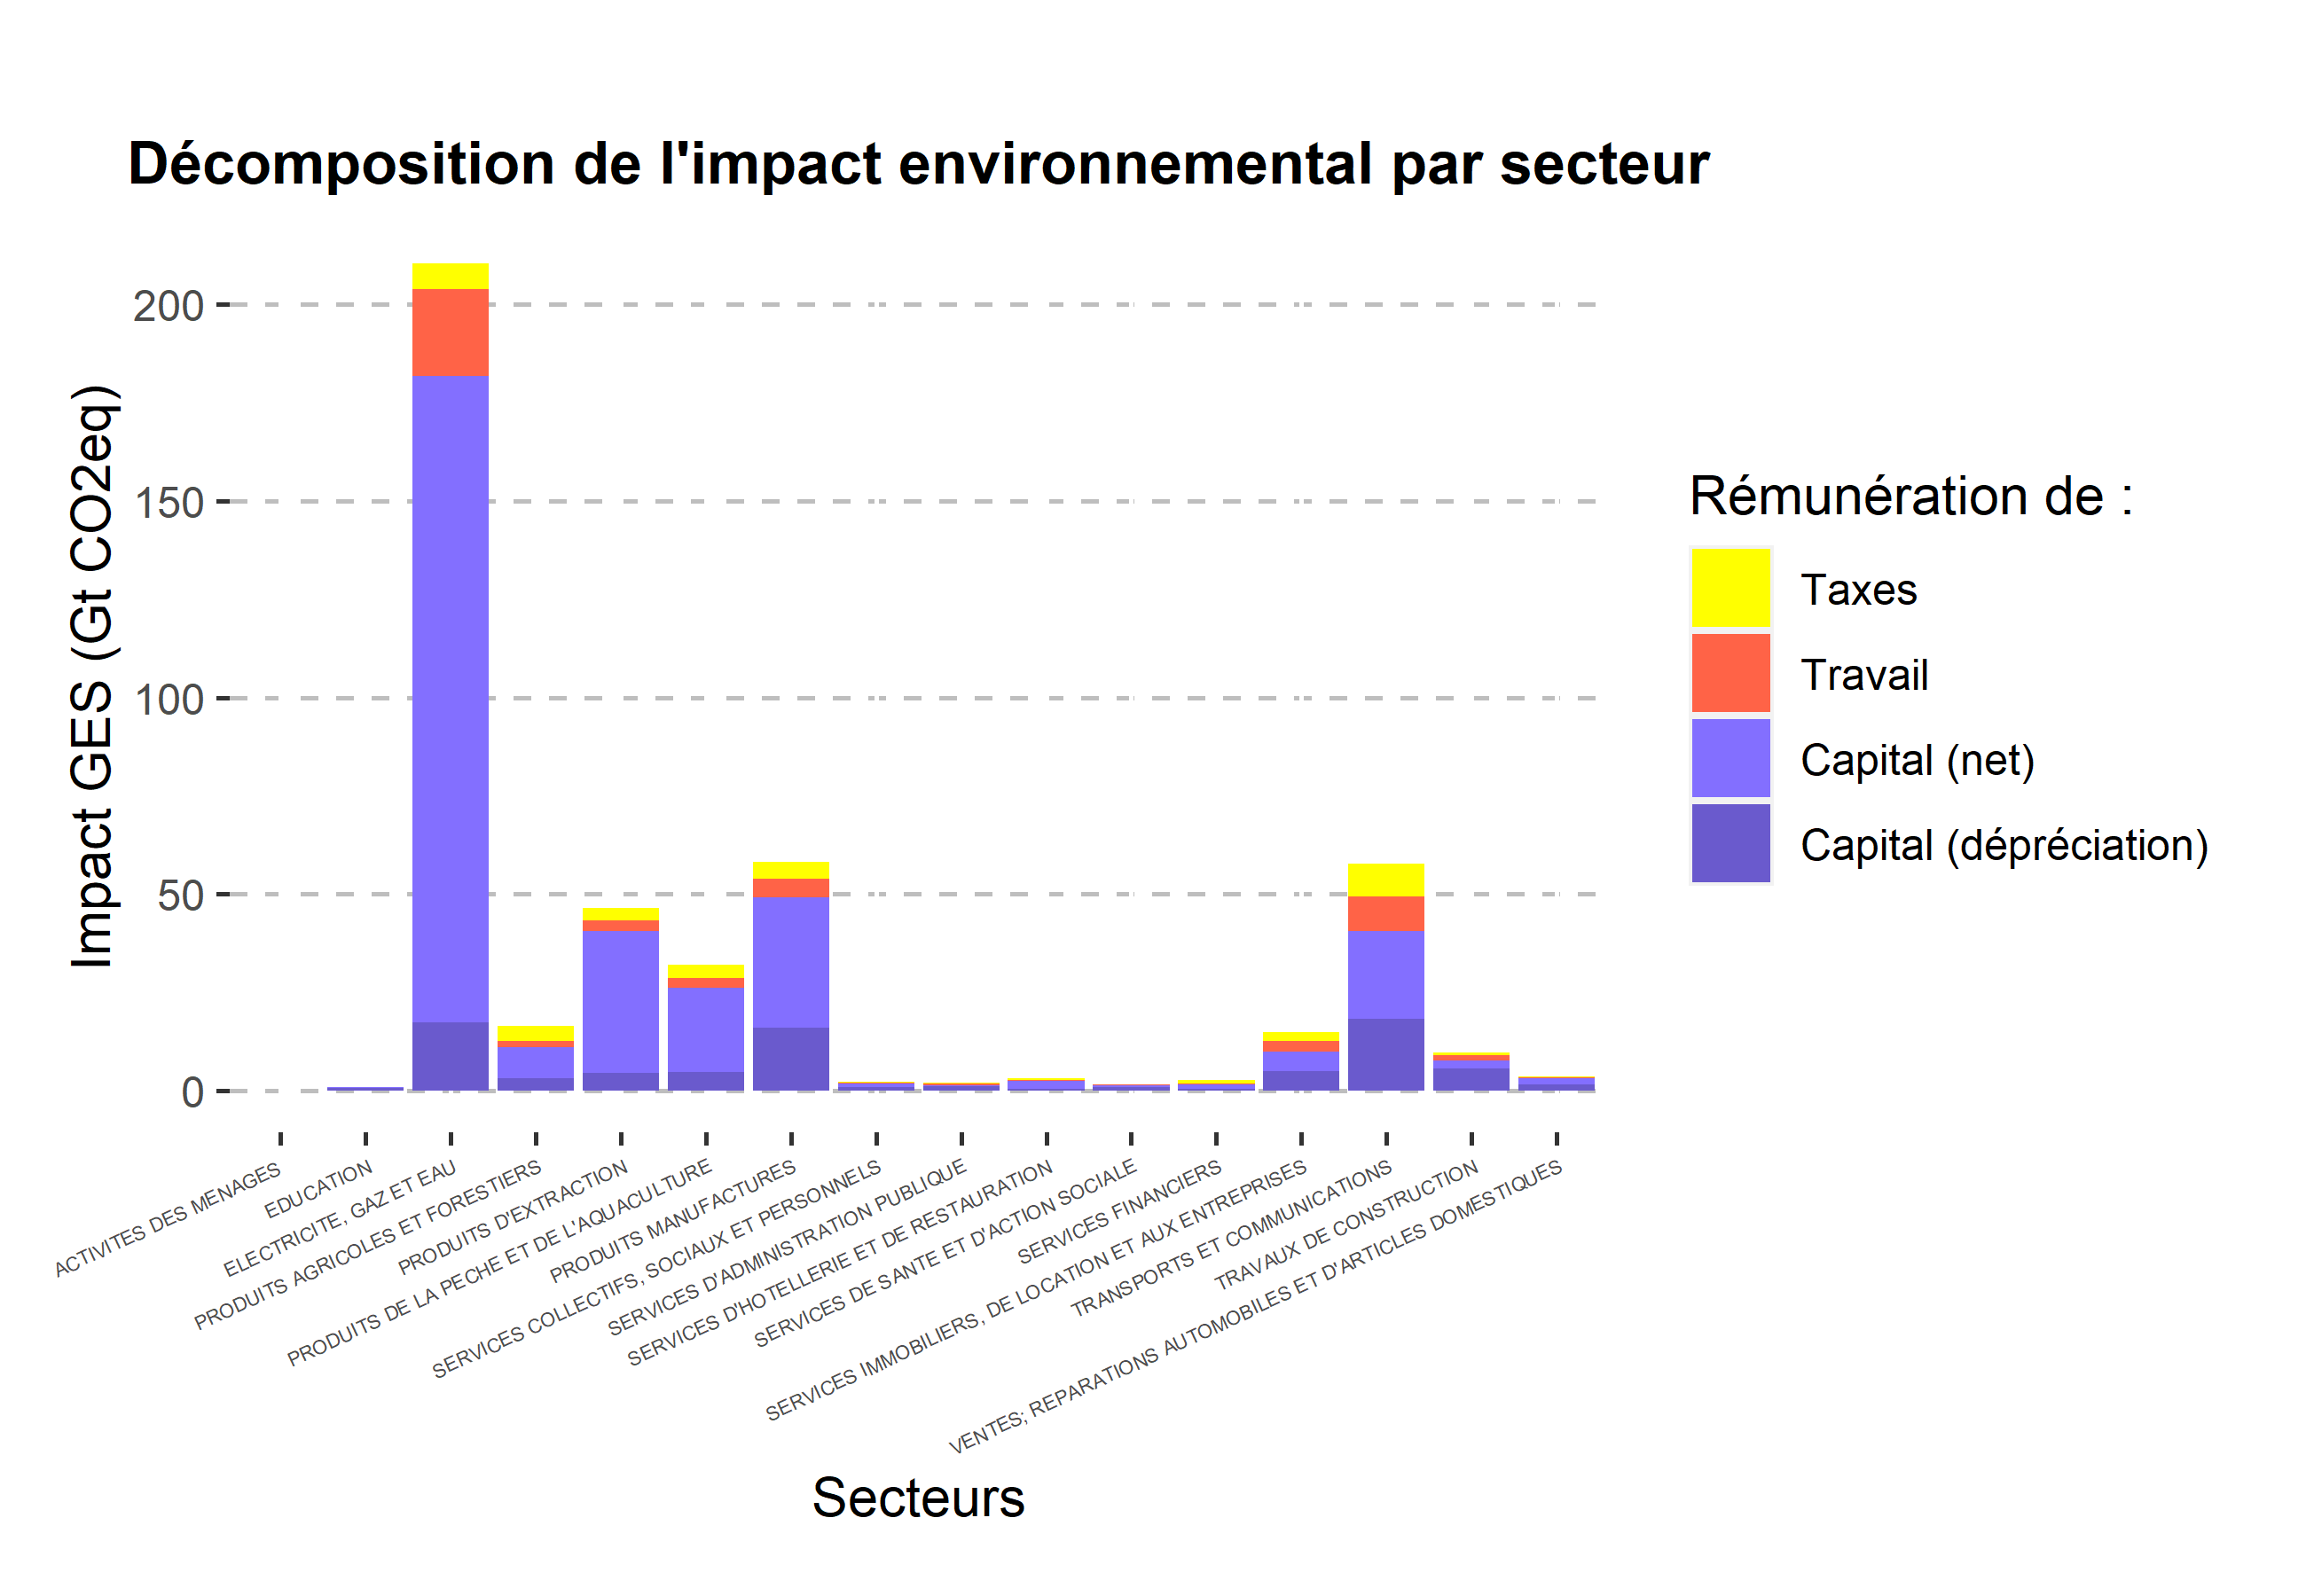
\includegraphics{resultatsEU2_files/figure-latex/monde secteurs impact-1.png}
\caption{Des inégalités d'impacts qui varient selon l'approche choisie}
\end{figure}

The value-added-based indicator can be decomposed into several
components. This allows to see which production factors contribute the
most to GHG emissions.

Capital is usually the largest contributor. Only in three instance does
the capital amout for (slighly) less than half of the emissions created:
``ELECTRICITE, GAZ ET EAU'', ``PRODUITS D'EXTRACTION'' and ``SERVICES
IMMOBILIERS, DE LOCATION ET AUX ENTREPRISES''. In the two latter cases,
the share of taxes in VA is remarkably large (more than 1/4)

\hypertarget{focus-on-europe-and-the-european-union}{%
\subsection[Focus on Europe and the European Union
]{\texorpdfstring{Focus on Europe and the European Union
\footnote{UK is included}}{Focus on Europe and the European Union }}\label{focus-on-europe-and-the-european-union}}

SECTEURS EUROPE SEULEMENT SI GROSSE DIFFERENCE AVEC MONDE

\begin{verbatim}
## # A tibble: 2 x 4
##   binaire agg.demande_impact agg.producteur_impact agg.VA_impact
##   <chr>                <dbl>                 <dbl>         <dbl>
## 1 EU                    3.58                  3.07          3.07
## 2 Reste                26.4                  27.0          27.0
\end{verbatim}

Avant de détailler comment se répartissent les impacts environnementaux
au sein de l'Union Européenne, on situe celle-ci par rapport au reste du
monde.

L'impact en gaz à effets de serre de l'Union Européenne est bien moindre
que celui du reste du monde (RDM), quel que soit l'indicateur choisi.
L'impact de la demande du RDM est 7 fois plus élevé que celui de la
demande européenne, l'impact de la production du RDM est 9 fois plus
élevé que celui de la production européenne, l'impact des revenus du RDM
est plus de 3 fois supérieur à celui des revenus européens.

\hypertarget{stylized-facts-at-the-european-scale}{%
\subsubsection{Stylized facts at the european
scale}\label{stylized-facts-at-the-european-scale}}

\begin{figure}
\centering
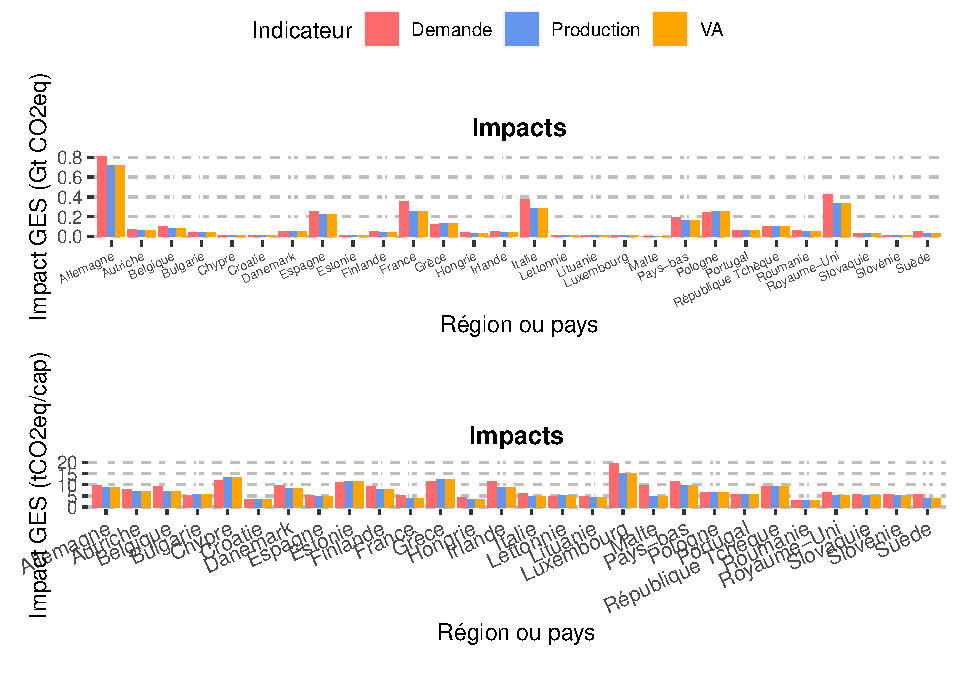
\includegraphics{resultatsEU2_files/figure-latex/EU pays-1.pdf}
\caption{D'importantes disparités}
\end{figure}

Dans l'Union Européenne, la plupart des pays sont nets demandeurs
d'émissions. L'Union dans son ensemble est également nette demandeuse
d'émissions (le reste du monde produit plus d'émissions qu'il n'en
demande). Certains pays européens sont nets producteurs (la Bulgarie,
Chypre, l'Estonie, la Grèce, la Pologne, le Portugal, la République
Tchèque) mais la différence n'est flagrante que pour quatre d'entre eux.

L'Allemagne a de loin le plus fort impact selon les trois approches.

Les petits pays et certains pays d'Europe du Nord ont le plus faible
impact (Chypre, Malte, le Luxembourg, la Croatie, l'Estonie, la
Lettonie, la Lituanie).

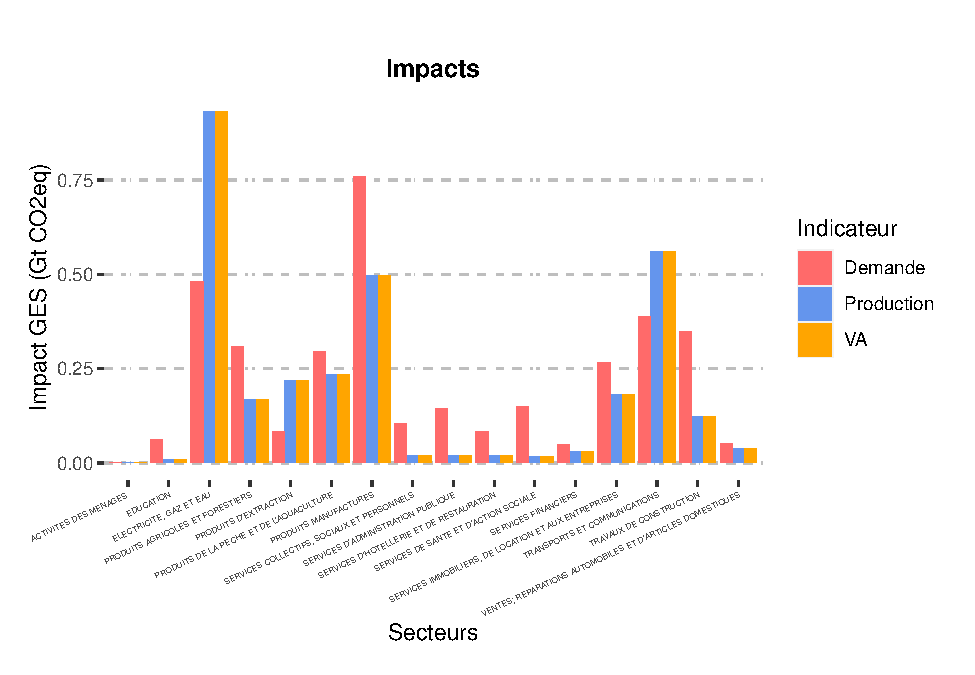
\includegraphics{resultatsEU2_files/figure-latex/EU secteurs-1.pdf}

Dans une approche sectorielle, le plus fort contraste entre secteurs
s'observe au niveau de l'impact producteur. Le secteur ``ELECTRICITE,
GAZ ET EAU'' se détache nettement avec le plus fort impact producteur,
suivi par les ``PRODUITS MANUFACTURES''.

Le plus fort impact demande concerne les secteurs ``PRODUITS
MANUFACTURES'', ``SERVICES IMMOBILIERS, DE LOCATION ET AUX ENTREPRISES''
et ``TRAVAUX DE CONSTRUCTION''.

Enfin, les secteurs des ``SERVICES IMMOBILIERS, DE LOCATION ET AUX
ENTREPRISES'' et des ``PRODUITS MANUFACTURES'' ont le plus fort impact
revenus.

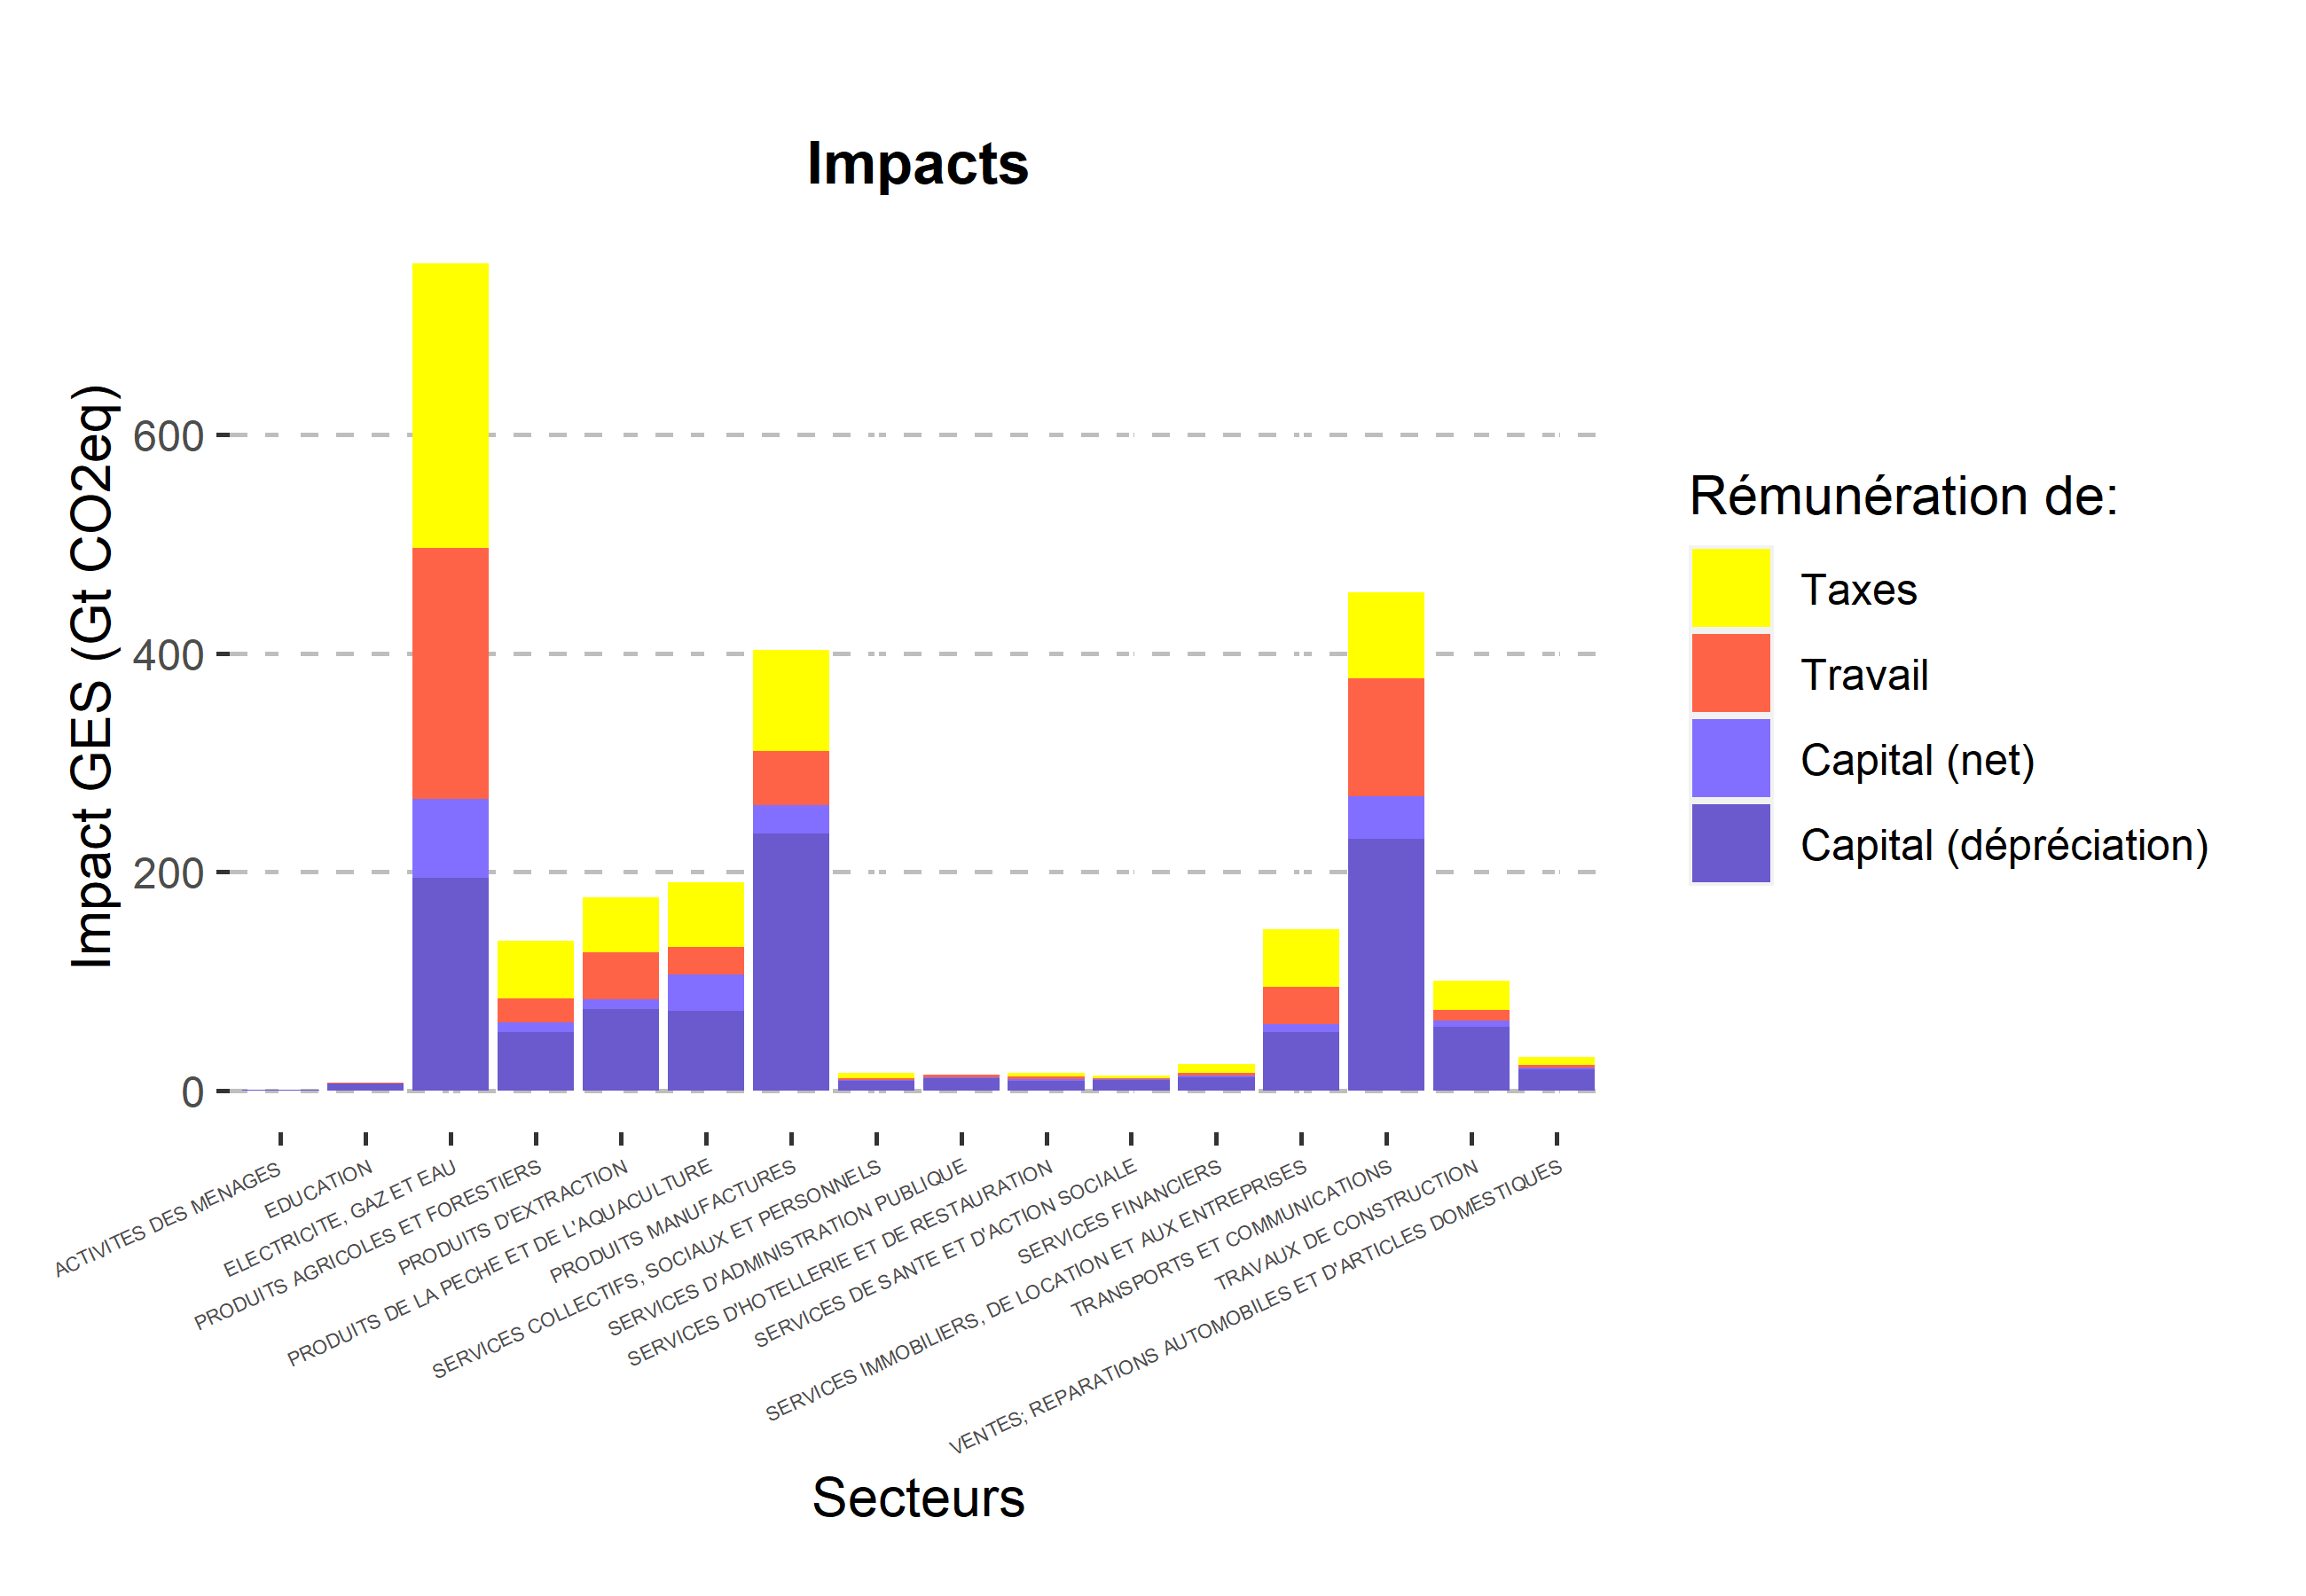
\includegraphics{resultatsEU2_files/figure-latex/monde secteurs va-1.png}

Globalement, parmi les facteurs de production c'est le capital fixe qui
a le plus fort impact. L'impacts du capital est le plus petit en
proportion pour chaque secteur.

\hypertarget{contrastes-par-pays}{%
\subsubsection{Contrastes par pays}\label{contrastes-par-pays}}

\includegraphics{resultatsEU2_files/figure-latex/groupes pays eu pib-1.pdf}

\includegraphics{resultatsEU2_files/figure-latex/groupes pays eu pop-1.pdf}

On voit également des contrastes à l'échelle régionale. L'Europe de
l'Ouest et du Sud ont le plus fort impact. Ces deux régions sont
également très hétérogènes, au contraire de l'Europe de l'Est et du Sud
dont les impacts sont plus homogènes entre pays. Les pays d'Europe de
l'Est sont généralement désavantagés par l'approche producteur (approche
selon lauelle ils ont le plus fort impact) alors que les autres sont
généralement désavantagés par l'approche valeur ajoutée.

EX FIGURE Le graphique ci-dessus montre à quel point chaque secteur
peut-être avantagé ou désavantagé par l'approche choisie : il représente
la part de chaque approche dans l'impact total d'un secteur.

En ce qui concerne la répartition des impacts selon l'approche adoptée,
il semble y avoir une corrélation positive entre la part de l'impact de
la demande et la part de l'impact créé par la valeur ajoutée. Il y a
aussi une corrélation négative entre la part de ces deux impacts, et la
part de l'impact producteur.

Deux secteurs ressortent particulièrement: ``ELECTRICITE, GAZ ET EAU''
et ``PRODUITS D'EXTRACTION'' ont à la fois le plus faible impact demande
et revenu en proportion, et la plus forte part d'impact producteur. Le
secteur ``ACTIVITES DES MENAGES'' est le plus avantagé par l'approche
producteur et le plus désavantagé par l'approche revenus.

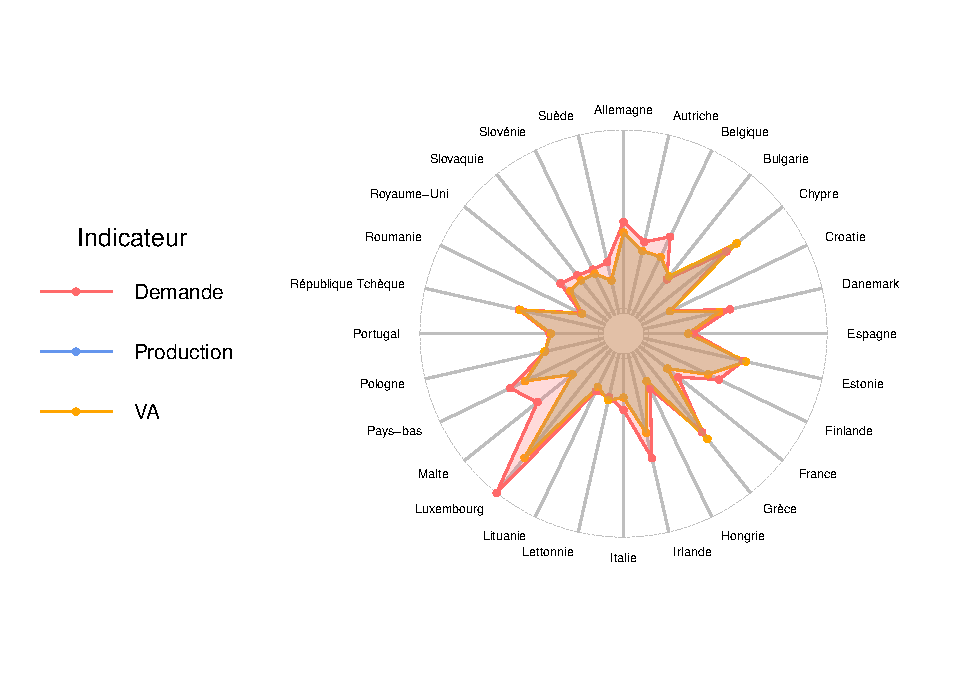
\includegraphics{resultatsEU2_files/figure-latex/parts impacts pays-1.pdf}

EX FIGURE\_PAYS Le graphique ci-dessus permet de tirer le même type de
conclusions mais au niveau des pays, et non des secteurs.

Le constat n'est pas le même: il semble plutôt y avoir une corrélation
positive entre le fait d'être avantagé par l'approche demande et le fait
d'être avantagé par l'approche production ; et une corrélation négative
entre le fait d'être avantagé par ces deux approches et par l'approche
revenus. L'exemple typique est la Suède : c'est à la fois le pays qui
est le plus avantagé par les indicateurs demande et producteur, et celui
qui est le plus désavantagé par l'indicateur valuer ajoutée (son impact
est 5 fois plus grand selon l'indicateur valeur ajoutée que selon
l'indicateur production).

L'hétérogénéité semble moins forte que dans l'approche sectorielle.
L'approche par la demande semble traiter les pays européens de la façon
la plus égalitaire (sans tenir compte ici du niveau de richesse, de la
taille du pays). L'approche valeur ajoutée est celle qui présente le
plus de disparités entre pays.

La conclusion est donc que selon qu'on adopte une approche
territoriale/nationale ou une approche sectorielle, la répartition des
coûts suit une logique différente.

\includegraphics{resultatsEU2_files/figure-latex/radar pays européens-1.pdf}
\includegraphics{resultatsEU2_files/figure-latex/radar pays européens-2.pdf}
\includegraphics{resultatsEU2_files/figure-latex/radar pays européens-3.pdf}

In most cases, Value added is the most emissions-intensive (also makes
sense because ). From one country to another, the most
emissions-intensive sector is not the same. In France ``PRODUITS
D'EXTRACTION'' is the most intensive (all three indicators).
``ELECTRICITE, GAZ ET EAU'' is the most intensive sector in Germany (by
far) and in Spain.

\hypertarget{conclusion}{%
\subsection{Conclusion}\label{conclusion}}

REFLECHIR A L'ORDRE DES AXES SUR RADAR

CHANGER UNITES DES GRAPHS (V)

NORMALISER PAR POPULATION (V)

PAR UNITE PRODUITE (V)

EDIT GRAPH VA (AUSSI AJOUTER GRAPH NORMALISE PAR EURO DE VA) (V)

AJOUTER UN RADAR PAR PAYS OU CHAQUE AXE EST UN SECTEUR (PE CHOISIR QQUES
PAYS POUR LE DOC) (V)

GROUPES DE PIB PAR HABITANT AU LIEU DE REGIONS, TROIS OU QUATRE
CATEGORIES (V)

DIAGONALISER POUR TROUVER LES VOLUMES DE LA BONNE DIMENSION (V)

FAIRE LES RADARS AVEC LES MULTIPLICATEURS PLUTOT QUE VOLUMES (V)

\end{document}
